\documentclass[greek]{beamer}
%\usepackage{fontspec}
\usepackage{amsmath,amsthm}
\usepackage{unicode-math}
\usepackage{xltxtra}
\usepackage{graphicx}
\usetheme{CambridgeUS}
\usecolortheme{seagull}
\usepackage{hyperref}
\usepackage{ulem}
\usepackage{xgreek}

\usepackage{pgfpages}
\usepackage{tikz}
\usepackage{tkz-tab}
%\setbeameroption{show notes on second screen}
%\setbeameroption{show only notes}

\setsansfont{Noto Serif}

\usepackage{multicol}

\usepackage{appendixnumberbeamer}

\setbeamercovered{transparent}
\beamertemplatenavigationsymbolsempty

\title{Τριγωνομετρία}
\subtitle{Τριγωνομετρικοί Αριθμοί - Ακτίνια - Τριγωνομετρικός Κύκλος}
\author[Λόλας]{Κωνσταντίνος Λόλας}
\date{}

\begin{document}

\begin{frame}
 \titlepage
\end{frame}

\section{Θεωρία}
\begin{frame}{Απλή εφαρμογή ακτινίων}
 \begin{itemize}
  \item<1-> Τι είναι το 1 ακτίνιο?
  \item<2-> Τι είναι τα 2 ακτίνια?
  \item<3-> Τι είναι τα 4.1 ακτίνια?
  \item<4-> Τι είναι τα $α$ ακτίνια?
 \end{itemize}
 \begin{block}{Μήκος Τοξου}<5->
  Το τόξο $α$ ακτινίων ενός κύκλου ακτίνας $ρ$ έχει μήκος
  $$S=αρ$$
 \end{block}
 \onslide<6-> Άσκηση 3 σχολικού
\end{frame}

\section{Ασκήσεις}
\subsection{Άσκηση 1}
\begin{frame}[label=Άσκηση1]{Εξάσκηση 1}
 Να υπολογίσετε τους τριγωνομετρικούς αριθμούς της γωνίας $ω$ που φαίνεται στο σχήμα

 \centering
 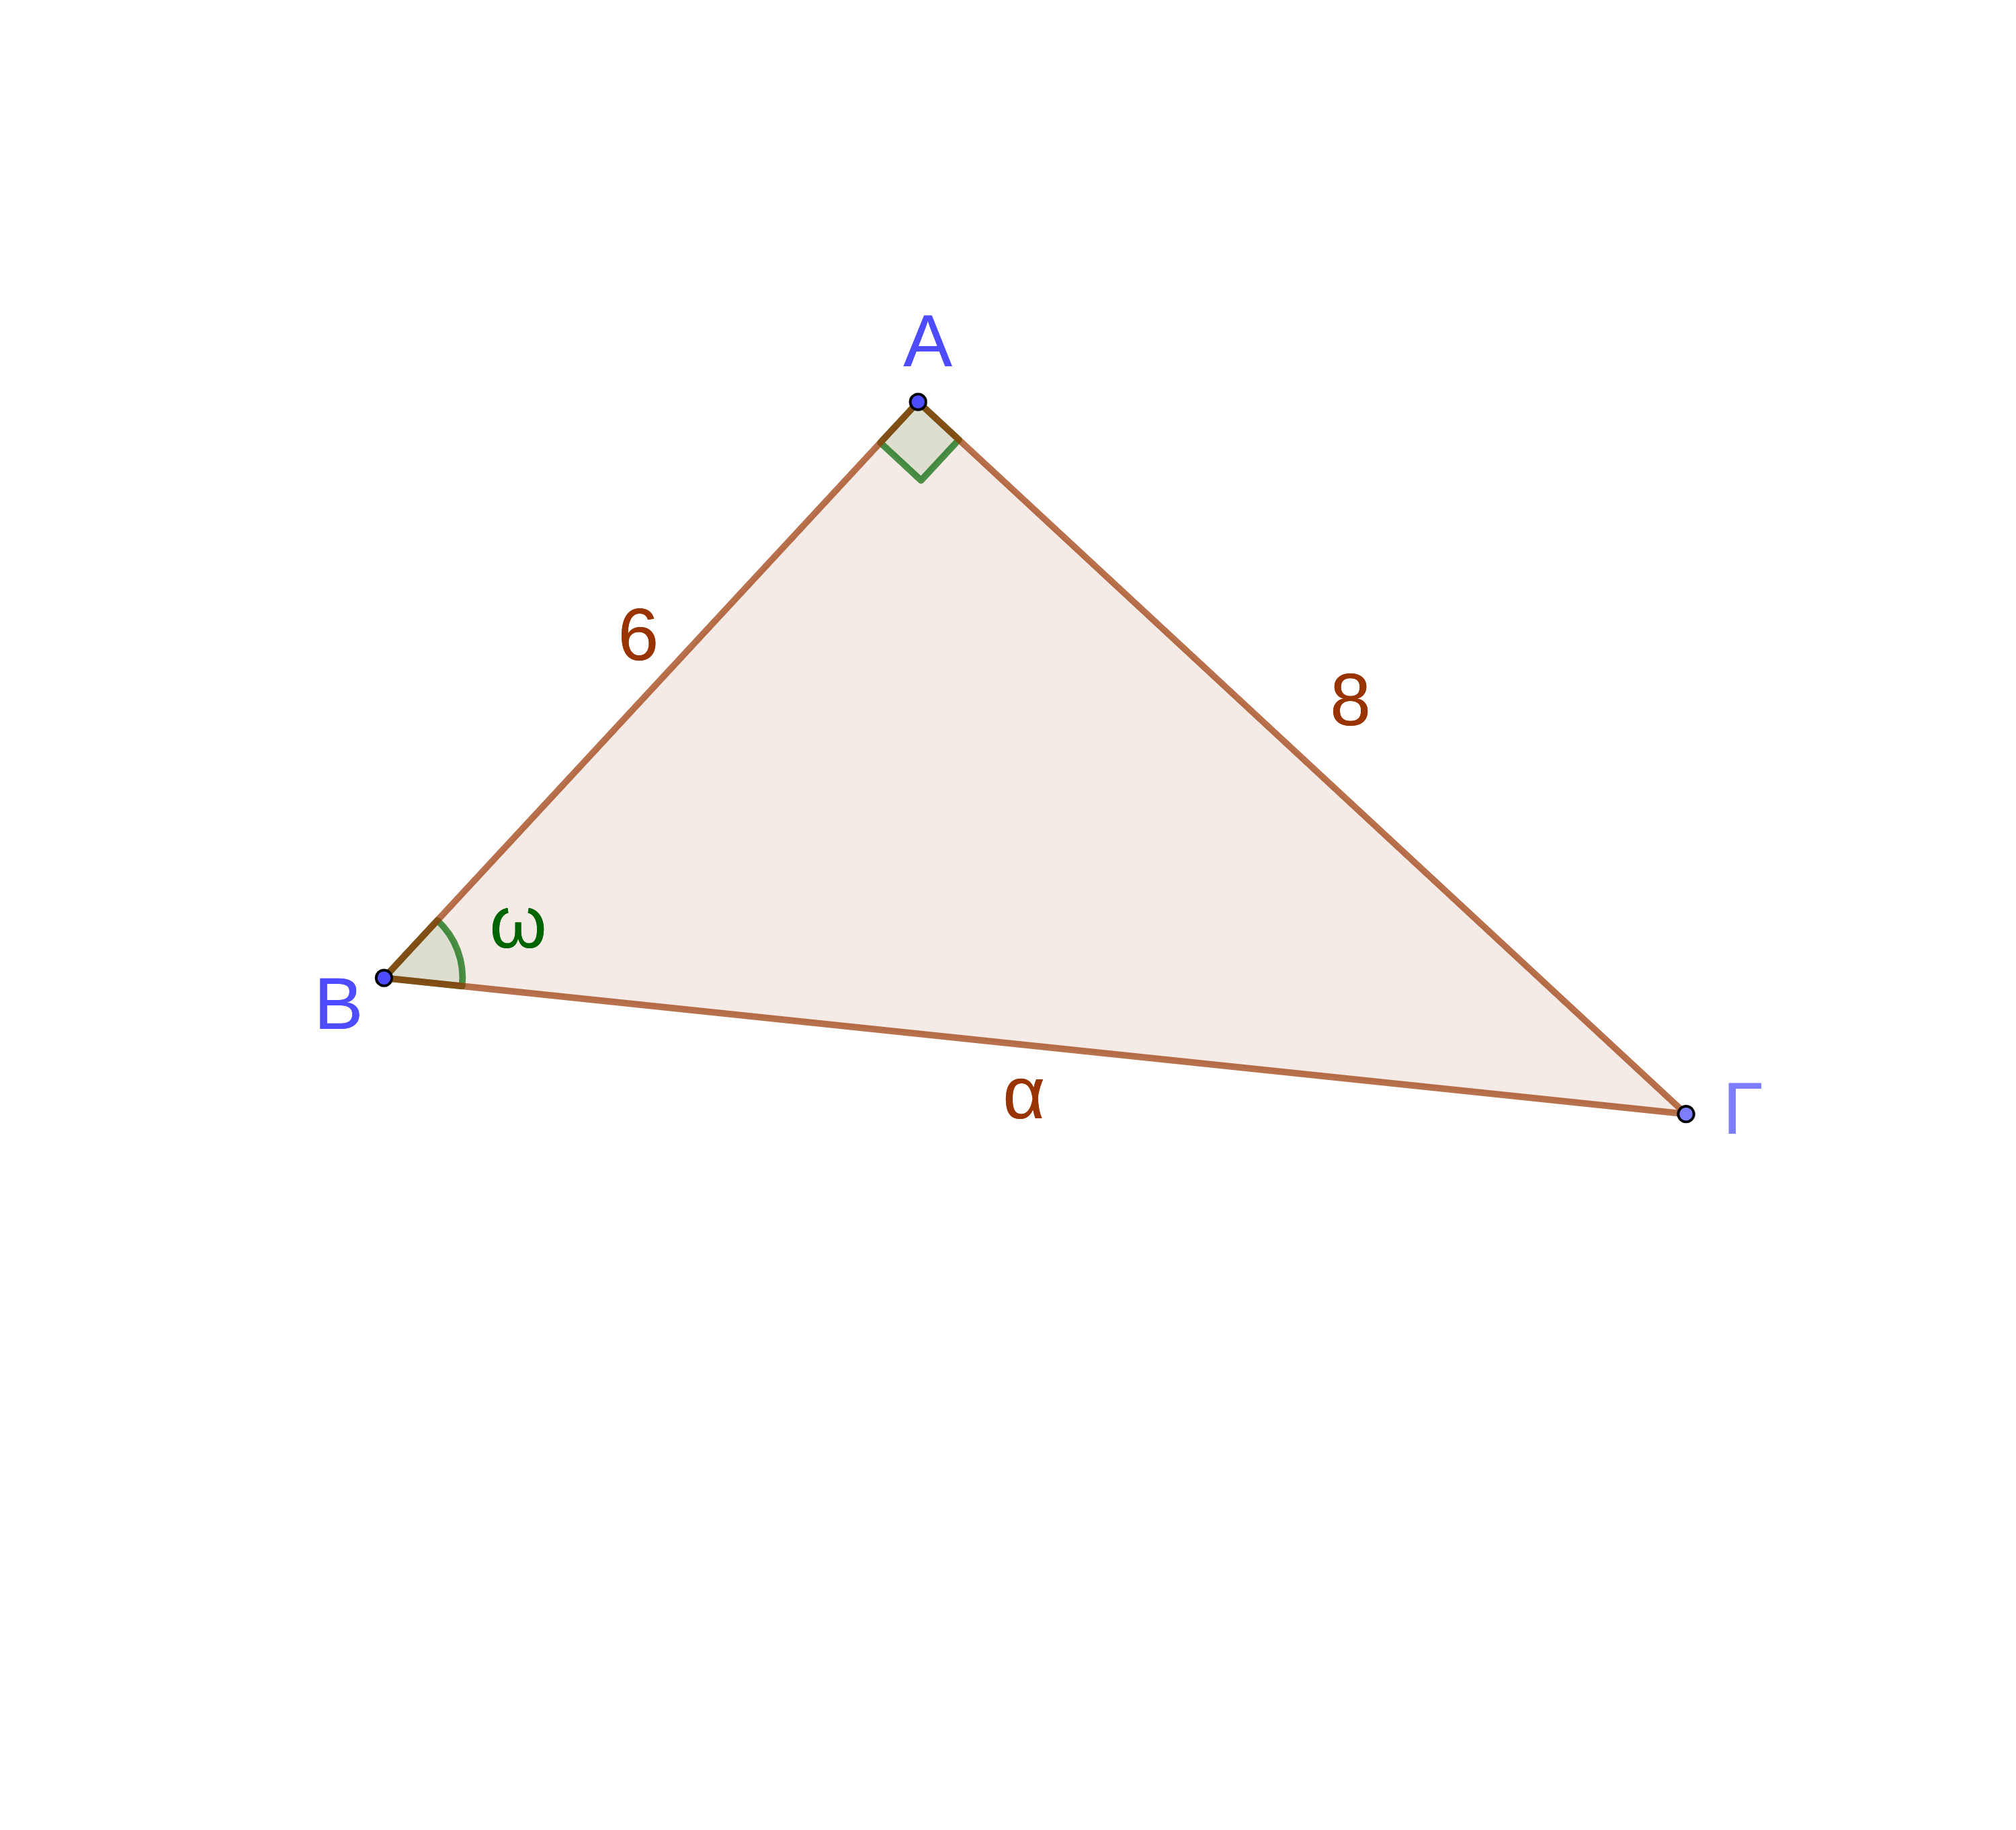
\includegraphics[width=0.8\textwidth]{"./images/3.1.1_1.png"}

 % \hyperlink{Λύση1}{\beamerbutton{Λύση}}
\end{frame}

\subsection{Άσκηση 2}
\begin{frame}[label=Άσκηση2]{Εξάσκηση 2}
 Στο σχήμα είναι $συνω=\frac{8}{17}$. Να βρείτε το $x$ και την $εφω$

 \centering
 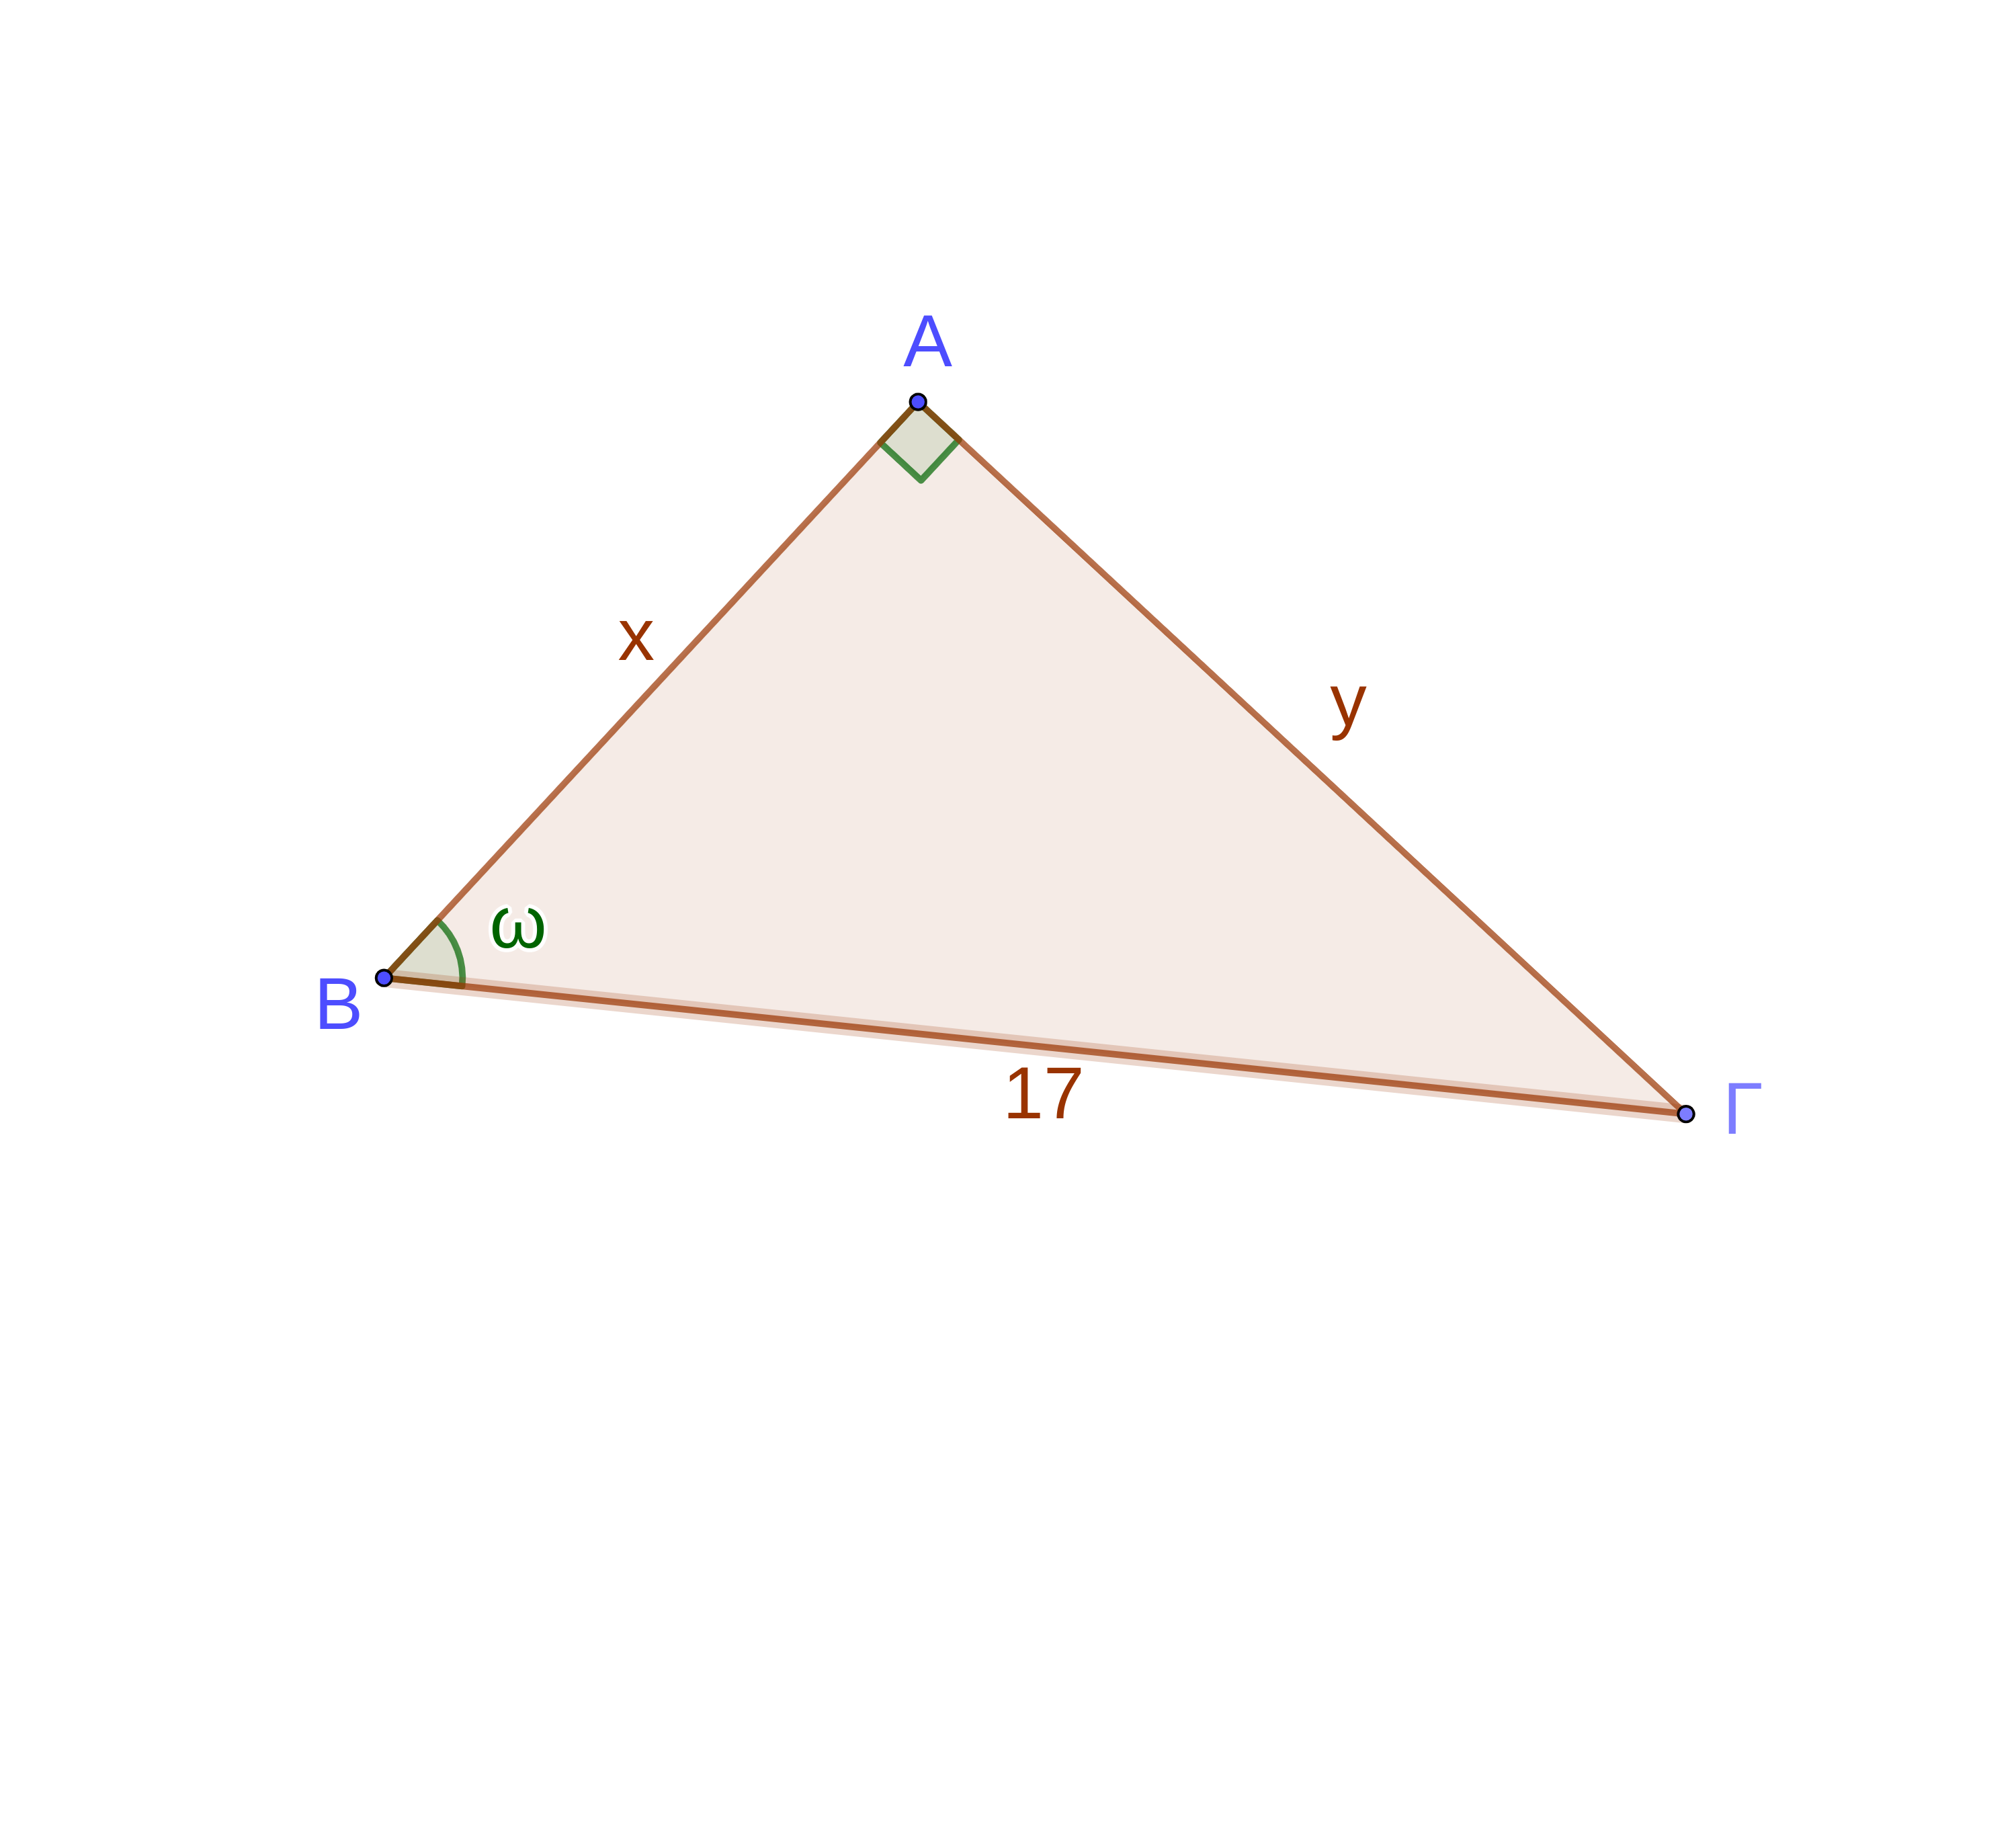
\includegraphics[width=0.8\textwidth]{"./images/3.1.1_2.png"}


 %\hyperlink{Λύση2}{\beamerbutton{Λύση}}
\end{frame}

\subsection{Άσκηση 3}
\begin{frame}[label=Άσκηση3]{Εξάσκηση 3}
 Στο σχήμα, να υπολογίσετε τα $x$ και $y$. Δίνονται $συν20^{\circ}=0.94$, $ημ20^{\circ}=0.34$ και $συν36^{\circ}=0.81$

 \centering
 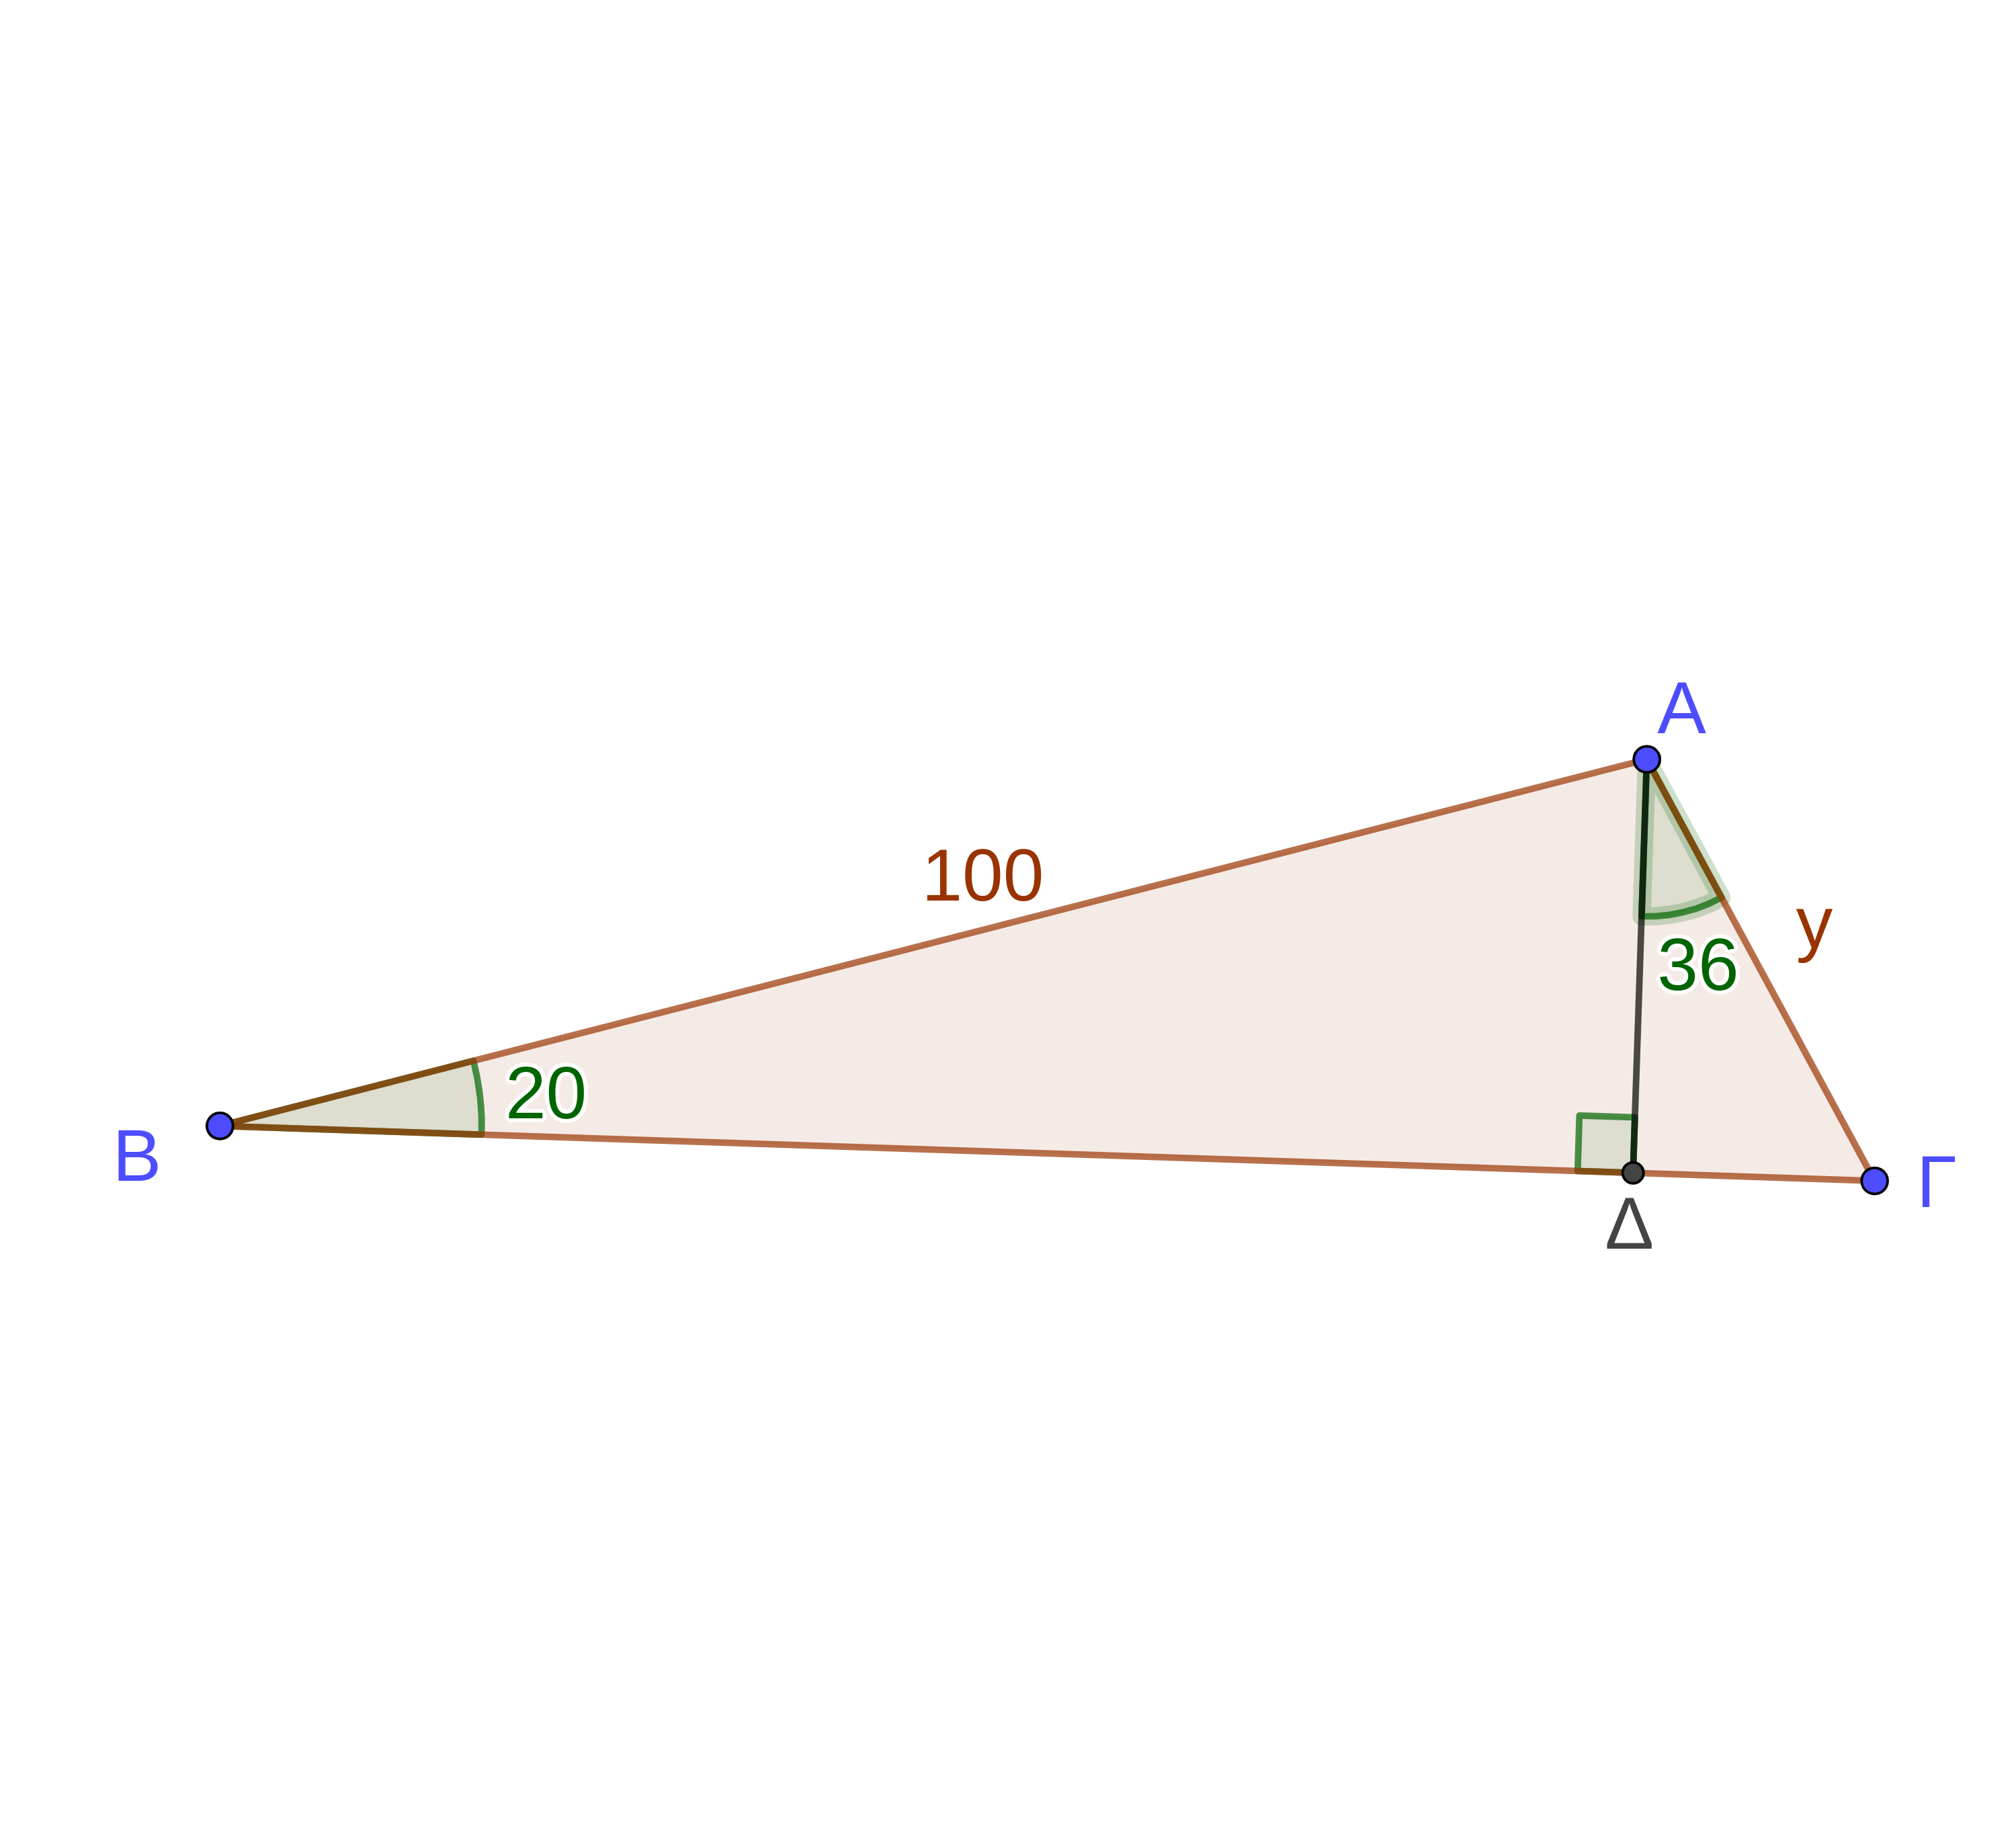
\includegraphics[width=0.8\textwidth]{"./images/3.1.1_3.png"}

 %\hyperlink{Λύση3}{\beamerbutton{Λύση}}
\end{frame}

\subsection{Άσκηση 4}
\begin{frame}[label=Άσκηση4]{Εξάσκηση 4}
 Μια επίκεντρη γωνία $ω$ βαίνει σε τόξο μήκους $S=20cm$. Να εκφράσετε τη γωνία $ω$ σε ακτίνια, αν η ακτίνα του κύκλου είναι $ρ=5cm$.

 %\hyperlink{Λύση4}{\beamerbutton{Λύση}}
\end{frame}

\subsection{Άσκηση 5}
\begin{frame}[label=Άσκηση5]{Εξάσκηση 5}
 Να εκφράσετε τη γωνία
 \begin{itemize}
  \item<1-> $120^{\circ}$ σε rad
  \item<2-> $\frac{3π}{4}$ rad σε μοίρες
 \end{itemize}

 %\hyperlink{Λύση5}{\beamerbutton{Λύση}}
\end{frame}

\subsection{Άσκηση 6}
\begin{frame}[label=Άσκηση6]{Εξάσκηση 6}
 Να υπολογίσετε την τιμή των παραστάσεων:
 \begin{itemize}
  \item<1-> $Α=ημ90^{\circ}-συν60^{\circ}+σφ45^{\circ}-συν180^{\circ}$
  \item<2-> $Β=ημ\frac{π}{6}-συν^2\frac{π}{6}-εφ\frac{π}{4}\cdot σφ\frac{π}{2}$
 \end{itemize}

 %\hyperlink{Λύση6}{\beamerbutton{Λύση}}
\end{frame}

\subsection{Άσκηση 7}
\begin{frame}[label=Άσκηση]{Εξάσκηση 7}
 Να υπολογίσετε τους τριγωνομετρικούς αριθμούς των γωνιών
 \begin{itemize}
  \item<1-> $765^{\circ}$
  \item<2-> $\frac{5π}{2}$ rad
  \item<3-> $\frac{49π}{6}$ rad
 \end{itemize}

 %\hyperlink{Λύση}{\beamerbutton{Λύση}}
\end{frame}

\subsection{Άσκηση 8}
\begin{frame}[label=Άσκηση8]{Εξάσκηση 8}
 Να βρείτε το πρόσημο των παραστάσεων:
 \begin{itemize}
  \item<1-> $Α=ημ100^{\circ}-συν200^{\circ}-εφ1000^{\circ}$
  \item<2-> $Β=ημ1-συν2$
  \item<3-> $Γ=συν3 \cdot εφ5$
 \end{itemize}

 %\hyperlink{Λύση8}{\beamerbutton{Λύση}}
\end{frame}

\subsection{Άσκηση 9}
\begin{frame}[label=Άσκηση9]{Εξάσκηση 9}
 Να βρείτε το πρόσημο των παραστάσεων:
 \begin{itemize}
  \item<1-> $Α=συν^2x-συνx-εφx$, $x\in (\frac{π}{2},π]$
  \item<2-> $Β=συν\frac{x}{2}+ημ2x-συν3x$, $\frac{π}{4}<x<\frac{π}{2}$
 \end{itemize}

 %\hyperlink{Λύση9}{\beamerbutton{Λύση}}
\end{frame}

\subsection{Άσκηση 10}
\begin{frame}[label=Άσκηση10]{Εξάσκηση 10}
 Να βρείτε μεταξύ ποιων αριθμών βρίσκονται οι τιμές των παραστάσεων:
 \begin{itemize}
  \item<1-> $Α=2-5ημx$
  \item<2-> $Β=3-2συν^2x$
  \item<3-> $Γ=\frac{1}{5-2ημx}$
 \end{itemize}

 %\hyperlink{Λύση10}{\beamerbutton{Λύση}}
\end{frame}

\section{}
\begin{frame}
 Στο moodle θα βρείτε τις ασκήσεις που πρέπει να κάνετε, όπως και αυτή τη παρουσίαση
\end{frame}

% \appendix
% \section{Λύσεις Ασκήσεων}
% \begin{frame}
%  \tableofcontents
% \end{frame}

\end{document}
